The primary result of this project is a dataset of synthetic images generated using Unity, offering an alternative to real-world images for training and testing machine learning models. The dataset consists of XXXX images with various boats and maritime objects in a harbor environment. It showcases the capabilities of the Unity Perception package, including the use of diverse scenarios with varying camera positions, weather effects, and object orientations. These features increase the dataset's diversity for machine learning tasks, helping to create better models.

\section{Dataset}
The dataset comprises synthetic images depicting objects in a harbor environment, generated entirely using Unity. Objects in the dataset include boats, sailboats, kayaks, buoys, and windsurfers, with variations in environmental conditions such as rain.\\

\noindent The distribution of object types and their corresponding weather conditions is summarized in Table~\ref{tab:dataset_composition}. Each object type has been rendered under various conditions to ensure a realistic and comprehensive dataset for training machine learning algorithms.
 
\begin{table}[H]
\centering
\begin{tabular}{|l|c|c|}
\hline
\multicolumn{3}{|c|}{\textbf{Dataset Distribution}} \\ 
\hline
\textbf{Object Type} & \textbf{Total Images} & \textbf{Rainy Images} \\ 
\hline
Boat         & 1,000  & 20  \\ 
Sailboat     & 300    & 20  \\ 
Kayak        & 100    & 50  \\ 
Buoy         & 200    & 50  \\ 
Windsurfer   & 200    & 50  \\ 
\hline
\textbf{Total}       & \textbf{1,800} & \textbf{190} \\ 
\hline
\end{tabular}
\caption{Breakdown of the dataset by object type and weather condition.}
\label{tab:dataset_composition}
\end{table}



\begin{figure}[H]
\centering
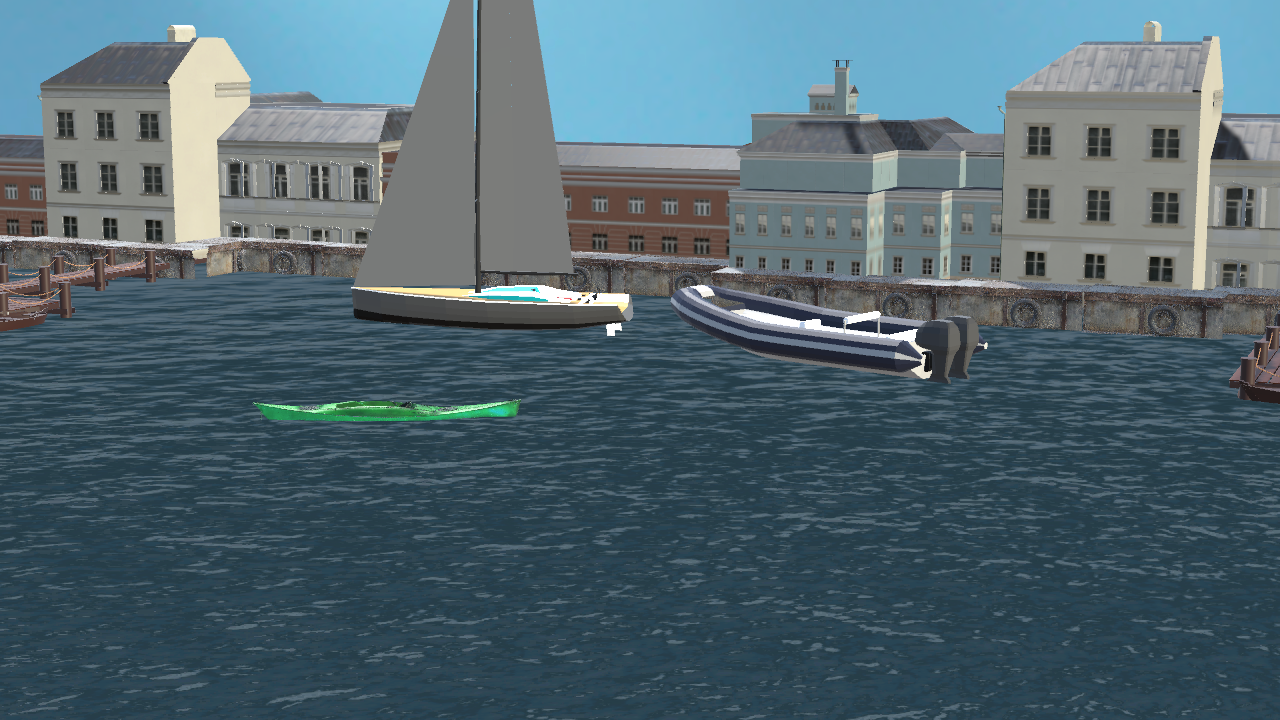
\includegraphics[width=0.8\textwidth]{Figures/results/rand2.png}
\caption{Example of one of the images in the dataset}
\label{fig:original_image}
\end{figure}

\section{Dataset Diversity}
A key goal of this project was to create a dataset that reflects many different scenarios. Using Unity's Perception package, randomization was applied to make the dataset more varied. Changes in object rotations, positions, and weather conditions were included to ensure the dataset is general and helps models perform well in different situations.\\

\noindent Figure \ref{fig:randomized_images} shows examples of randomized images with the same target object. These examples highlight how randomization creates variety in rotation, background and camera position.

\begin{figure}[H]
\centering
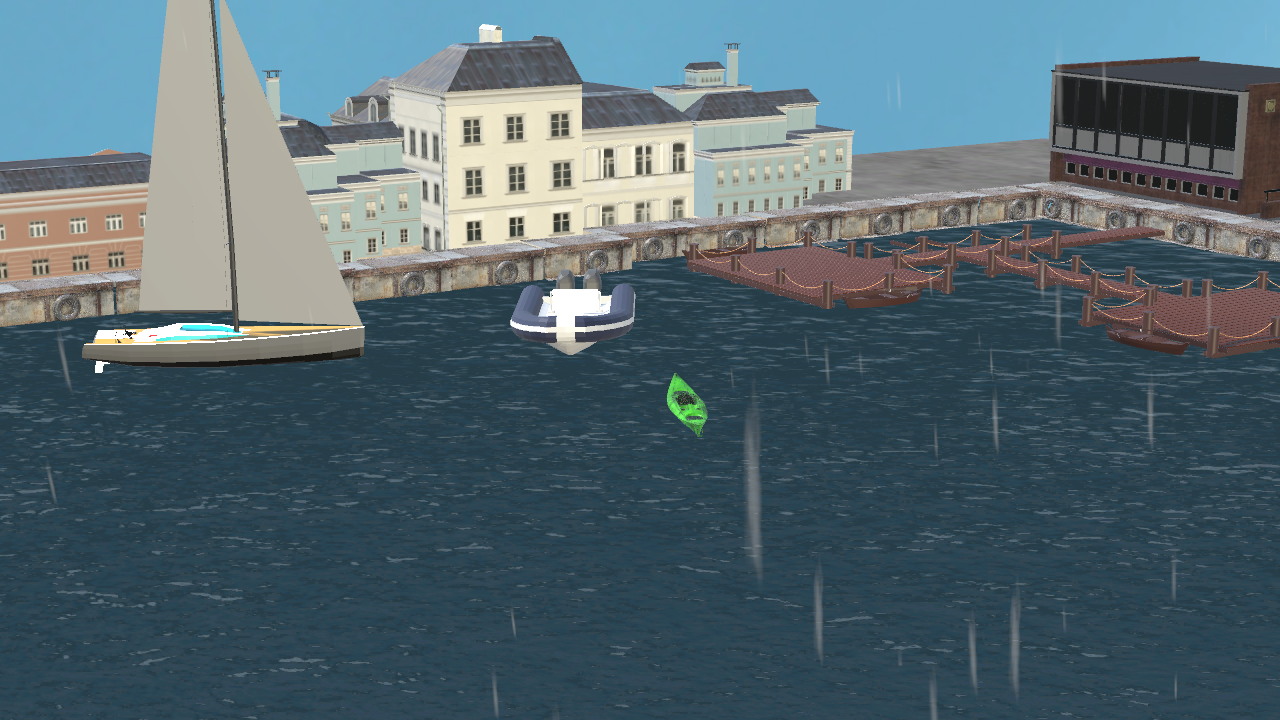
\includegraphics[width=0.32\textwidth]{Figures/results/rand1.png}
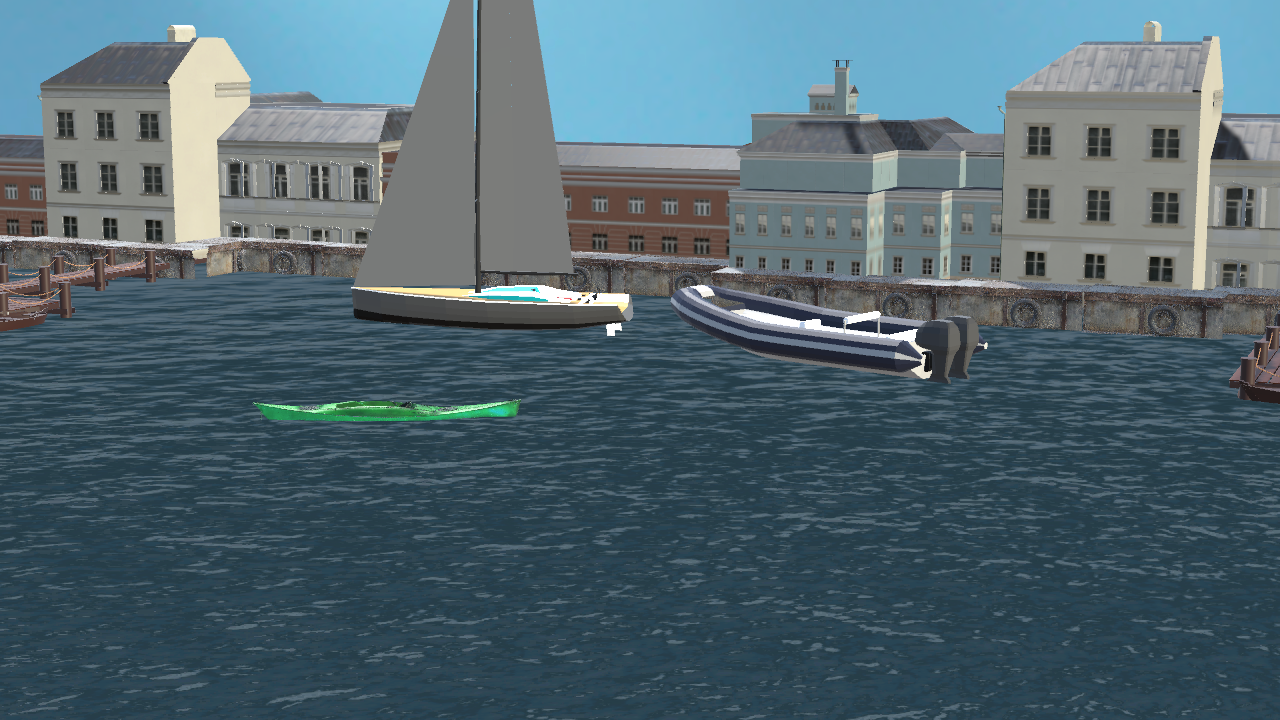
\includegraphics[width=0.32\textwidth]{Figures/results/rand2.png}
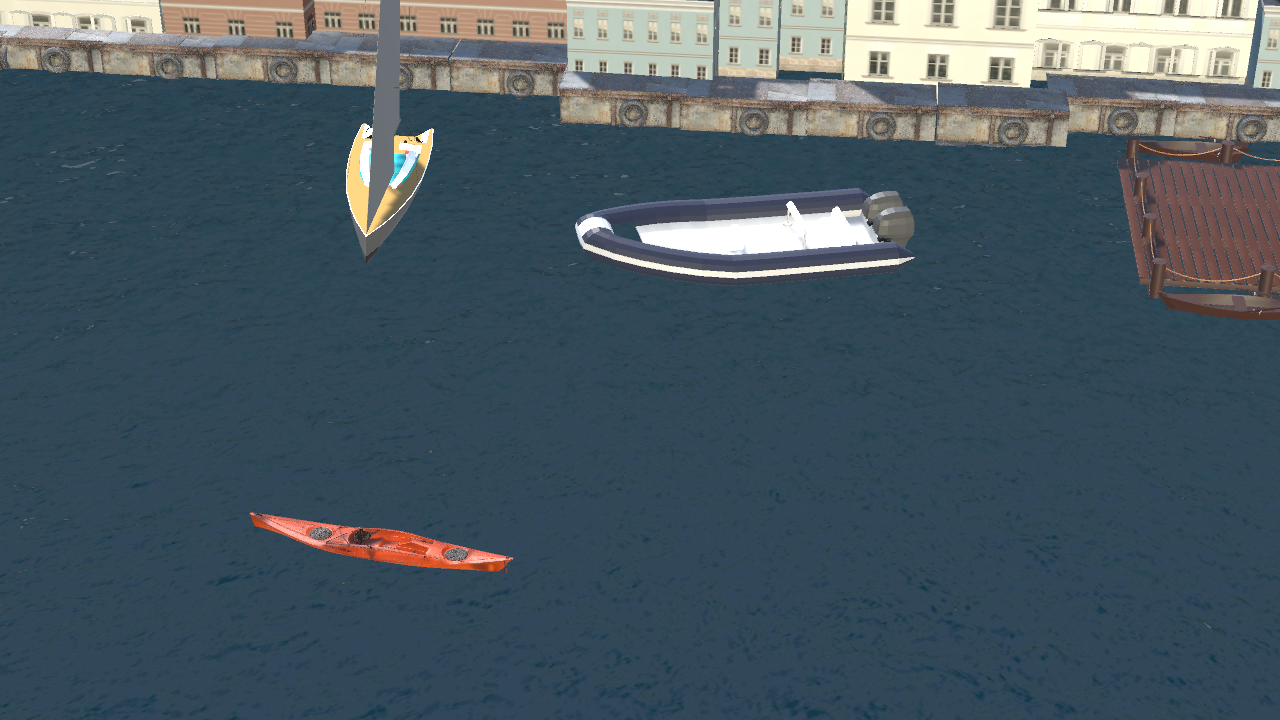
\includegraphics[width=0.32\textwidth]{Figures/results/rand3.png}
\caption{Example of 3 randomized images with the same target.}
\label{fig:randomized_images}
\end{figure}

\section{Labeling}
Labeling is important because it helps computer vision models identify and learn the objects in an image\cite{Labelling}. The Unity Perception package was used to automate this process, generating two images for each scene: the original image and a corresponding segmentation image.\\

\noindent Figure \ref{fig:labeled_images} shows an example of the labeling process. The left image is the original, and the right image is the segmented version. This comparison shows how well the labels match the objects in the original image, ensuring the model learns from accurate data.

\begin{figure}[H]
\centering
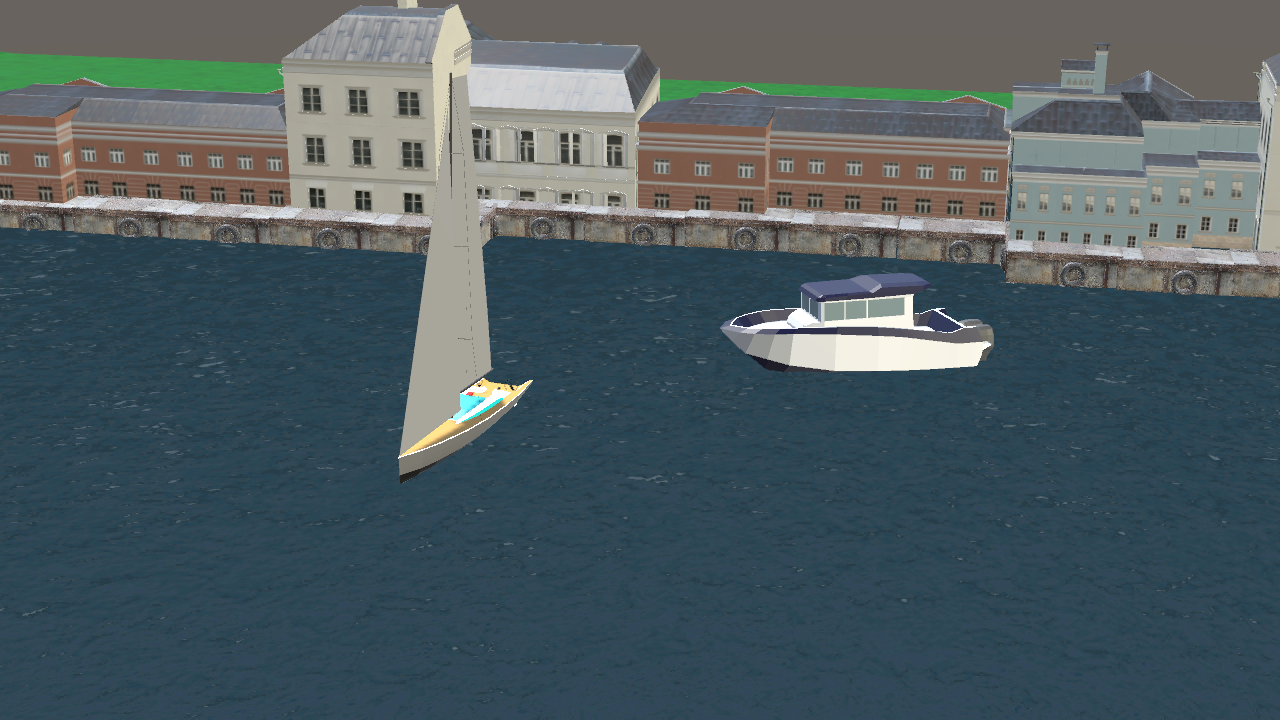
\includegraphics[width=0.49\textwidth]{Figures/rgb_2.png}
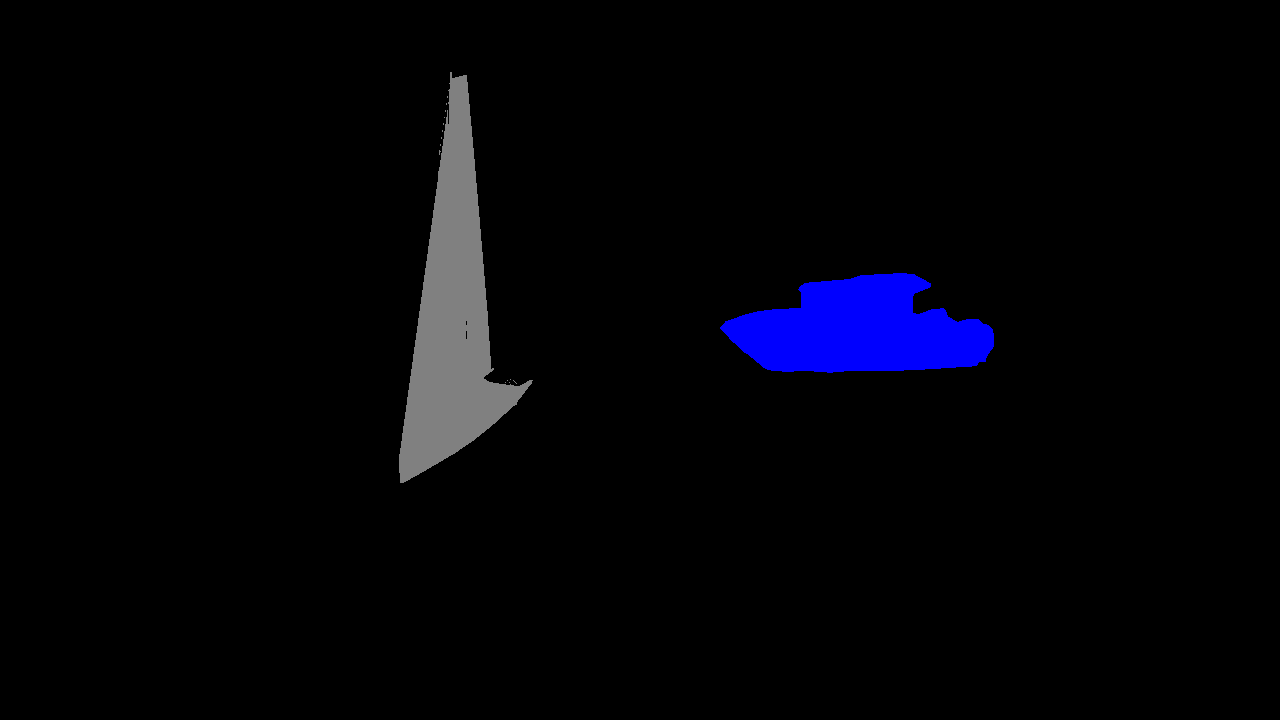
\includegraphics[width=0.49\textwidth]{Figures/segmentation_2.png}
\caption{Comparison of the original image and its labeled segmentation output.}
\label{fig:labeled_images}
\end{figure}

\section{Discussion}
Overall, the results of this project have been positive. A large number of images were generated, and the environment was designed to make it quick and easy to produce even more images if needed. However, there are areas where improvements could enhance the dataset’s effectiveness for machine learning applications.

\subsection{Realism of the 3D Models and Environment}
The quality of the generated images was limited by the free assets used in the project. While the water simulation contributed to a sense of realism, other elements, such as docks and boats, relied on low-poly models. Low-poly models are simpler and less detailed than high-poly ones, which significantly impacted the overall realism of the scenes. \\

\noindent This lack of detail could reduce the suitability of the dataset for tasks requiring high levels of photorealism. For instance, sharp edges and visible simplicity in some objects made it easy to spot the artificiality of the scenes. This domain gap between synthetic and real-world data could pose challenges when applying models trained on this dataset to real-world environments.

\subsubsection{Techniques to Bridge the Domain Gap}
There are several techniques available to enhance the realism of the dataset and reduce the domain gap, such as:

\begin{itemize}
\item \textbf{Texture Replacement}: Using higher-resolution textures to improve the visual fidelity of objects.
\item \textbf{Post-Processing}: Applying tools like Unity's Post-Processing Stack to simulate effects such as motion blur, depth of field, and color grading.

\end{itemize}

\subsubsection{Combining AI with Unity for Enhancement}
A particularly promising approach is combining synthetic environments with AI-based tools to improve image realism. For example, Stable Diffusion, accessed via the Dezgo platform, was used to enhance Unity-generated images by adding photorealistic details. In addition to improving realism, AI-enhanced images introduce subtle variations to the scenes, such as altering the appearance of boats or modifying the background. These enhancements not only make the dataset look more realistic but also increase its diversity, which is beneficial for training robust machine learning models.\\

\noindent Figure \ref{fig:ai_enhanced} illustrates the transformation of Unity-generated images after enhancement with AI tools. This post-processing step significantly improves the visual appeal and realism of the images, potentially making the dataset more effective for machine learning applications.

\begin{figure}[H]
\centering
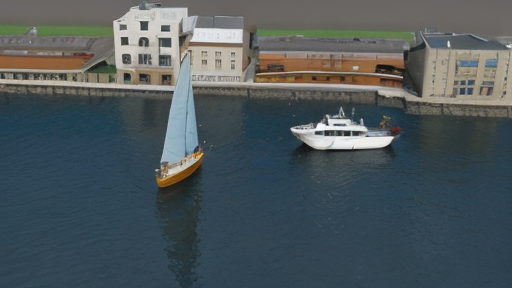
\includegraphics[width=0.49\textwidth]{Figures/results/photorealistic_3613113118.png}
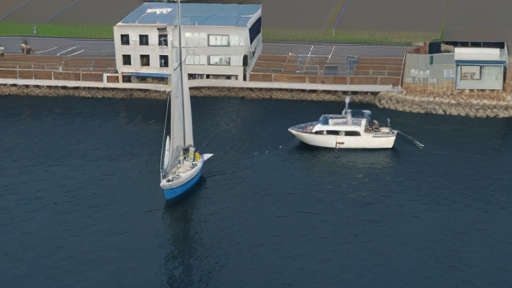
\includegraphics[width=0.49\textwidth]{Figures/results/photorealistic_2942539231.png}
\caption{AI-enhanced images generated using Dezgo.}
\label{fig:ai_enhanced}
\end{figure}

This method offers a pathway to creating high-quality synthetic datasets with minimal additional effort, which is worth exploring further in future projects or semesters.


\subsection{Expanding the Dataset}
Expanding the dataset is straightforward due to the flexibility of the setup. With the environment already built and the Unity Perception package\cite{unity-perception2022} integrated, additional images can be generated quickly and efficiently whenever needed. This capability ensures the dataset can grow whenever needed. \\

\noindent Another way to expand the dataset is by applying traditional augmentation techniques to the existing images. Techniques such as image rotation, flipping (mirroring), zooming, and cropping can introduce further variation without requiring additional 3D rendering. These methods enhance the diversity of the dataset and can improve the generalizability of machine learning models trained on it.

\subsection{Challenges and Limitations}
Several challenges arose during the project, particularly related to Unity's version compatibility and asset rendering. For instance, imported materials were sometimes incompatible with the project's Unity version, causing objects to appear pink or fail to render altogether. These issues were especially disruptive for water simulations, which limited the variety and realism of the scenes that could be created.\\

\noindent Additionally, the reliance on free or low-cost assets restricted the diversity and quality of objects available for use. This limitation not only reduced the range of scenarios represented in the dataset but also impacted the overall realism of the generated images.\\

\noindent To address these challenges, future projects could benefit from investing in higher-quality assets or collaborating with designers to develop custom 3D models tailored to specific needs. These improvements would enhance both the visual fidelity and the diversity of the dataset, making it more robust for training machine learning models.



